\documentclass[oneside]{book}
\usepackage{url,verbatim,fancyvrb}
\usepackage{pifont}
\usepackage[latin1]{inputenc}
\usepackage[pdftex]{graphicx}
%\usepackage[authoryear]{natbib}
\usepackage{color,gretl}
\usepackage[letterpaper,body={6.3in,9.15in},top=.8in,left=1.1in]{geometry}
\usepackage[pdftex,hyperfootnotes=false]{hyperref}
\usepackage{dcolumn,amsmath,bm}

\newcommand{\ttusage}[1]{\textit{example}: \quad \texttt{#1}}
\newcommand{\vbusage}[0]{\textit{example}: \quad}

%% \pdfimageresolution=120
\hypersetup{pdftitle={Gretl Function Package Guide},
            pdfsubject={Using and writing gretl function packages},
            pdfauthor={Allin Cottrell and Riccardo (Jack) Lucchetti},
            colorlinks=true,
            linkcolor=blue,
            urlcolor=red,
            citecolor=steel,
            bookmarks=true,
            bookmarksnumbered=true,
            plainpages=false
}

\begin{document}

\VerbatimFootnotes

\setlength{\parindent}{0pt}
\setlength{\parskip}{1ex}
\setcounter{tocdepth}{1}

%% titlepage

\thispagestyle{empty}

\begin{center}
\pdfbookmark[1]{Gretl Function Package Guide}{titlepage}

\gtitle{Gretl Function Package Guide}

{\large \sffamily
Allin Cottrell\\
Department of Economics\\
Wake Forest University\\

\vspace{20pt}
Riccardo (Jack) Lucchetti\\
Dipartimento di Scienze Economiche e Sociali\\
Universit� Politecnica delle Marche\\

\vspace{20pt}
\input date
}

\end{center}
\clearpage

%% end titlepage, start license page

\thispagestyle{empty}

\pdfbookmark[1]{License}{license}

\vspace*{2in}

Permission is granted to copy, distribute and/or modify this document
under the terms of the \emph{GNU Free Documentation License}, Version
1.1 or any later version published by the Free Software Foundation
(see \url{http://www.gnu.org/licenses/fdl.html}).

\cleardoublepage

%% end license page, start table of contents
\pdfbookmark[1]{Table of contents}{contents}

\pagenumbering{roman}
\pagestyle{headings}

\tableofcontents

\clearpage
\pagenumbering{arabic}
%\setcounter{chapter}{-1}

\chapter{Introduction}
\label{chap:intro}

\section{The purpose of function packages}
\label{sec:purpose}

The primary purpose of gretl function packages is to add estimators,
hypothesis tests or other analytical procedures to gretl's repertoire
of built-in procedures. While function packages may also be used for
other purposes (e.g.\ pedagogy, replication exercises), those made
available via the gretl server are expected to extend gretl's
functionality in non-trivial ways.

For an extended discussion of the rationale for such packages see
``Extending gretl: addons and bundles''.\footnote{Presented by Allin
  Cottrell at the 2011 gretl conference---see
  \url{http://gretl.sourceforge.net/papers/addons.pdf}.} Note,
however, that the distinction between regular packages and ``addons''
in that document has become somewhat blurred, as regular packages have
gradually acquired many of the rights and responsibilities previously
confined to official gretl ``addons''. On the rights side, regular
packages are now able to hook into the gretl GUI; on the
responsibilities side, contributed packages are now subject to
(minimal) vetting before they can appear in the public download area
on the gretl server.
  
\section{The form of function packages}
\label{sec:pkgform}

The core component of a gretl function package---in simpler cases,
the sole component---is a \textsf{gfn} file. This is an XML file
conforming to the Document Type Definition \texttt{gretlfunc.dtd},
which is supplied in the gretl distribution and can also be found in
gretl CVS.\footnote{See
  \url{http://gretl.cvs.sourceforge.net/viewvc/gretl/gretl/share/functions/gretlfunc.dtd?view=log}.}
Such files contain
\begin{itemize}
\item the hansl code for at least one function;
\item various items of metadata (author, version, date, etc.);
\item help text for the function(s), or a pointer to help in
  PDF format; and
\item a sample script that illustrates a call to the packaged
  function(s). 
\end{itemize}

While it is possible in principle to create and edit a \textsf{gfn}
file ``manually'', using a suitable text editor, this is not
recommended. Gretl provides tools (both command-line and GUI) to create
and maintain package files, such that authors are not required to
mess with raw XML.

We will refer to packages that consist of a gfn file alone as ``simple
packages'' (the included hansl code may not be simple, but the
structure is). 

The alternative to a simple package we will call a ``zip package''.
Such packages take the form of a \textsf{PKZIP} archive containing a
\texttt{gfn} file along with other materials, which may include PDF
documentation (in place of plain text help), data needed by the
package for internal use (for example, tables of critical values for
some test statistic), and/or extra data files or scripts intended to
supplement the required sample script. Zip packages can be built using
command-line tools or with the help of the gretl GUI.

One point to note about zip packages is that the \textsf{PKZIP}
wrapper is actually just a storage and transport format. When such a
package is installed, it is unpacked in a suitable location. Further
details on this package format can be found in
chapter~\ref{chap:zipfile}.

\section{Using this document}

Text wanted here.

\chapter{For package users}
\label{chap:users}

To be written: take in (updated) material from the User's Guide and/or
elsewhere.

\section{Acquiring a package}

Text wanted here.

\section{Using packages via the command line}

Text wanted here.

\section{Using packages via the GUI}

Text wanted here.

\chapter{For package authors}
\label{chap:authors}

``In the beginning was the command line'' (Neal Stephenson), so we'll
start with CLI methods for building a package. Those who prefer to use
a graphical interface whenever possible may skip ahead to
section~\ref{sec:gui-build}. However, the GUI interface for creating
function packages is likely to be convenient for small to medium-sized
packages but may be too cumbersome for ambitious packages that include
a large hierarchy of private functions. 

\section{Building a package via the command line}
\label{sec:cli-build}

First of all, we strongly recommend that when starting work on a
package you create a specific directory to hold the makings of the
package. For illustration we'll suppose the package is called
``mypkg''. (Naturally, you should replace all occurrences of
\texttt{mypkg} below with the actual name of the package you're
building.) So, starting from some suitable point in your file system,
you might begin with
%
\begin{code}
mkdir mypkg
cd mypkg
\end{code}

Now, the minimum requirement for building your package (as a ``simple
package'' or stand-alone \textsf{gfn} file) is the following set of
files:
\begin{itemize}
\item At least one (for now, let's just say one) hansl \textsf{inp}
  file containing definitions of the functions you wish to
  package. Let's call this \texttt{mypkg.inp}.
\item A \textsf{spec} file, which supplies metadata and tells gretl how the
  package should be assembled; call this \texttt{mypkg.spec}.
\item A sample script (\textsf{inp} file) which exercises your
  package; call this \texttt{mypkg\_sample.inp}.
\item A plain text file containing help on the packaged function(s);
  call this \texttt{mypkg\_help.txt}.
\end{itemize}

You will need to create such files in the current directory (or maybe
copy or move them from elsewhere if you've already made a start). It's
not absolutely necessary that \textit{all} the filenames are
regimented as shown (starting with the name of the package in each
case), but as we'll see before long this can make life easier.

The \textsf{inp} file containing your function definitions we won't
say much about here. If you're contemplating writing a package you
should already be pretty comfortable with hansl. See the \textit{Hansl
  Primer} if in doubt.\footnote{Look in
  \url{http://sourceforge.net/projects/gretl/files/manual/}.}

The requirements on the sample script and help text are set out in
section~\ref{sec:common-req}.  That leaves the \textsf{spec}
file. We'll approach this by stages, starting with the simplest
possible case (see Example~\ref{ex:spec1}).

\begin{script}[htbp]
  \caption{Simple \texttt{mypkg.spec}}
  \label{ex:spec1}
\begin{code}
author = A. U. Thor
email = author@somewhere.net
version = 1.0
date = 2015-07-12
description = Suitable description goes here
public = myfunc
help = mypkg_help.txt
sample-script = mypkg_sample.inp
min-version = 1.9.3
\end{code}
\end{script}

According to this spec, the package has a single public function,
\texttt{myfunc}, and requires gretl 1.9.3 or higher to run
properly. For details on all the specification keys (e.g.\
\texttt{min-version}) see chapter~\ref{chap:specfile}.

Now, assuming all the required files are in place, how do we actually
build the package? Simple: the shell command
%
\begin{code}
gretlcli --makepkg mypkg.inp
\end{code}
%
tells \textsf{gretlcli} to run \texttt{mypkg.inp}, hence loading your
function definitions into memory; read the corresponding \textsf{spec}
file (which must have the same basename as the \textsf{inp} file);
and, if all goes well, write out \texttt{mypkg.gfn} (FIXME: where?!).

We've said this package offers a single public function,
\texttt{myfunc}: that's the only function that will be made directly
available to users of the package. However, you may want to include
one or more private ``helper'' functions, designed to be called only
by \texttt{myfunc}. To do so, just put definitions of these functions
into \texttt{mypkg.inp}; \textsf{gretlcli} will pick them up and,
seeing that they don't appear in the \texttt{public} listing, will
mark them as private.


\section{Building a package via the GUI}
\label{sec:gui-build}

Here is a walk-through of the process.

\subsection{Load a function in memory}

There are several ways to load a function:

\begin{itemize}
\item If you have a script file containing function definitions, open
  that file and run it.
\item Create a script file from scratch.  Include at least one
  function definition, and run the script.
\item Open the GUI console and type a function definition
  interactively.  This method is not particularly recommended; you are
  probably better composing a function non-interactively.
\end{itemize}

For example, suppose you decide to package a function that returns the
percentage change of a time series. Open a script file and type
\begin{code}
function series pc(series y "Series to process")
    series ret = 100 * diff(y)/y(-1)
    string dsc = sprintf("Percentage change of %s", argname(y))
    setinfo ret --description="@dsc"
    return ret  
end function
\end{code}
In this case, we have appended a string to the function argument, so
as to make our interface more informative.  This is not obligatory: if
you omit the descriptive string, gretl will supply a predefined one.

\begin{figure}[htbp]
  \centering
  \begin{scode}
              x         dpcx

 1    0.4428625             
 2    0.3737993     -15.5947
 3    0.1570864     -57.9757
 4    0.6896227     339.0086
 5    0.8510148      23.4030
 6      0.07757     -90.8851
 7    0.1454557      87.5180
 8    0.8260684     467.9174
 9    0.4328073     -47.6064
10    0.3566473     -17.5967

  \end{scode}
  \caption{Output of function check}
  \label{fig:func_check}
\end{figure}

Now run your function. You may want to make sure it works properly by
running a few tests. For example, you may open the console and type

\begin{code}
genr x = uniform()
genr dpcx = pc(x)
print x dpcx --byobs
\end{code}

You should see something similar to figure \ref{fig:func_check}. The
function seems to work ok.  Once your function is debugged, you
may proceed to the next stage.

\subsection{Create a package}

We first present the mechanism for creating a function package via
gretl's graphical interface. This can also be done via the
command line, which offers some additional functionality for package
authors; an explanation is given later in this section.

Start the GUI program and take a look at the ``Tools, Function
packages'' menu.  This menu contains four items: ``On local machine'',
``On server'', ``Edit package'', ``New package''.

Select ``New package''.  (This will produce an error message unless at
least one user-defined function is currently loaded in memory---see
the previous point.)  In the first dialog you get to select:

\begin{itemize}
\item A public function to package.
\item Zero or more ``private'' helper functions.
\end{itemize}

Public functions are directly available to users; private functions are
part of the ``behind the scenes'' mechanism in a function package. So,
at this point, you select the \cmd{pc} function from the left-hand
panel and put it into the ``Public functions'' box.

\begin{figure}[htbp]
  \centering
  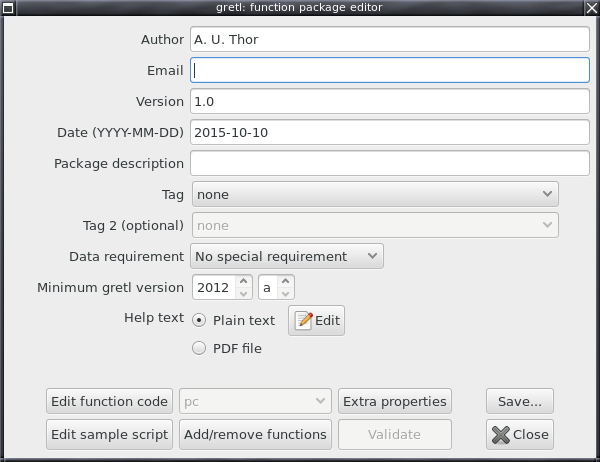
\includegraphics[scale=0.5]{figures/package_editor}
  \caption{The package editor window}
  \label{fig:package_editor}
\end{figure}

On clicking ``OK'' a second dialog should appear (see
Figure~\ref{fig:package_editor}), where you get to enter the package
information (author, version, date, and a short description).  You can
also enter help text for the public interface.  You have a further
chance to edit the code of the function(s) to be packaged, by clicking
on ``Edit function code''.  (If the package contains more than one
function, a drop-down selector will be shown.)  And you get to add a
sample script that exercises your package.  This will be helpful for
potential users, and also for testing.  A sample script is required if
you want to upload the package to the gretl server (for which a
check-box is supplied).

You won't need it right now, but the button labeled ``Save as script''
allows you to ``reverse engineer'' a function package, writing out a
script that contains all the relevant function definitions.

Clicking ``Save'' in this dialog leads you to a File Save dialog.  All
being well, this should be pointing towards a directory named
\texttt{functions}, either under the gretl system directory (if
you have write permission on that) or the gretl user directory.
This is the recommended place to save function package files, since
that is where the program will look in the special routine for opening
such files (see below).

Needless to say, the menu item ``Tools, Function packages, Edit
package'' allows you to make changes to a local function package.

\subsection{Load a package}

Why package functions in this way?  To see what's on offer so far, try
the next phase of the walk-through.

Close gretl, then re-open it.  Now go to ``Tools, Function packages,
On local machine''. If the previous stage above has gone OK, you
should see the file you packaged and saved, with its short
description.  If you click on ``Info'' you get a window with all the
information gretl has gleaned from the function package.  If you click
on the ``View code'' icon in the toolbar of this new window, you get a
script view window showing the actual function code. Now, back to the
``Function packages'' window, if you click on the package's name, the
relevant functions are loaded into gretl's workspace, ready to be
called by clicking on the ``Call'' button.

After loading the function(s) from the package, open the GUI console.
Try typing \texttt{help foo}, replacing \texttt{foo} with the name of
the public interface from the loaded function package: if any help text
was provided for the function, it should be presented.

In a similar way, you can browse and load the function packages
available on the gretl server, by selecting ``Tools, Function
packages, On server''.

Once your package is installed on your local machine, you can use the
function it contains via the graphical interface as described above,
or by using the CLI, namely in a script or through the console. In the
latter case, you load the function via the \texttt{include} command,
specifying the package file as the argument, complete with the
\texttt{.gfn} extension.

\begin{figure}[htbp]
  \centering
  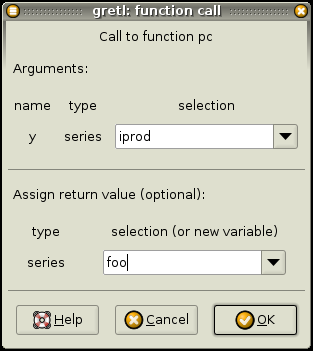
\includegraphics[scale=0.5]{figures/function_call}
  \caption{Using your package}
  \label{fig:function_call}
\end{figure}

To continue with our example, load the file \texttt{np.gdt} (supplied
with gretl among the sample datasets). Suppose you want to
compute the rate of change for the variable \texttt{iprod} via your
new function and store the result in a series named \texttt{foo}.

Go to ``Tools, Function packages, On local machine''.  You will be
shown a list of the installed packages, including the one you have
just created. If you select it and click on ``Execute'' (or
double-click on the name of the function package), a window similar to
the one shown in figure \ref{fig:function_call} will appear.  Notice
that the description string ``Series to process'', supplied with the
function definition, appears to the left of the top series chooser.

Click ``Ok'' and the series \texttt{foo} will be generated (see figure
\ref{fig:iprod_pc}).  Under some circumstances you might have to press
the ``r'' key (refresh) to have your new variable show up the main
window variable list.

\begin{figure}[htbp]
  \centering
  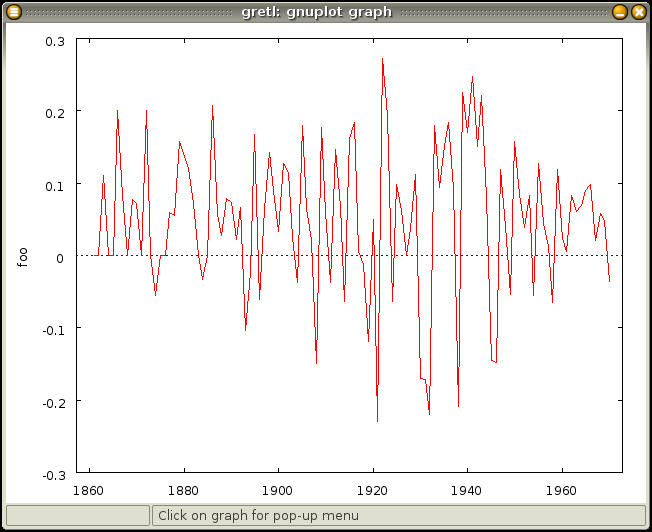
\includegraphics[scale=0.5]{figures/iprod_pc}
  \caption{Percent change in industrial production}
  \label{fig:iprod_pc}
\end{figure}

Alternatively, the same could have been accomplished by the script
\begin{code}
include pc.gfn
open np
foo = pc(iprod)
\end{code}


\section{Common requirements}
\label{sec:common-req}

Whether you're building a function package from the command line or
composing a package via the gretl GUI, certain requirements must be
met if your package is to be made available via the gretl server. Here
we spell out what's needed in regard to the help text and the sample
script.

\subsection{Help text}

This must give a clear (if brief) account, in English, of what the
package does, and also what each parameter does, for each public
function, insofar as explanation is reasonably required. (A boolean
\texttt{verbose} parameter probably doesn't need much if any comment,
but most parameters do need comment.)

If the help is not in PDF format (FIXME add cross-ref) it must be
encoded in UTF-8 (or plain ASCII, which is a proper subset of
UTF-8). We also recommend that lines of text are kept to close to 70
characters in width: some people may like to run gretl windows at
full-screen size, but many of us do not!

\subsection{Sample script}

This is crucial. The sample script \textit{must} work ``out of the
box'' on all platforms, and \textit{must not} take too long to
execute.

The sample script is what curious users are likely to run if they just
want to see what a package does and check that it's not broken. It's
what we package-checkers want to run for the same reasons, but also in
the process of regression-testing new gretl release candidates. It's
important that a new gretl release doesn't break existing packages,
but we can't assess that if a package's sample script is broken in the
first place.

Here are the key things to watch out for in relation to sample
scripts:
\begin{itemize}
\item \textbf{Include yourself}: Right at the top, the sample script
  must \texttt{include} the \texttt{gfn} file in question. This will
  never do any harm, and is needed when the script is run ``from
  scratch'', without the package being already loaded.  The name of
  the \texttt{gfn} file should be given without any added path, and
  without quotation marks, as in

  \texttt{include mypackage.gfn}

\item \textbf{Dataset}: If the package requires that a dataset be in
  place the sample script \textit{must} arrange for this in a portable
  manner. The options are as follows.
 \begin{enumerate}
 \item Open a data file that's supplied with the gretl distribution
   (that is, under the \textsf{Gretl}, \textsf{Greene} or
   \textsf{Ramanathan} tabs in the built-in datafile browser).
   But if none of the supplied data files are suitable, then
 \item construct an artificial dataset using the \texttt{nulldata}
   command and gretl's random-number generation facilities, or
 \item specify a downloaded data file using the \texttt{http} prefix
   with the \texttt{open} command; or
 \item include a suitable data file in your package---this requires
   that the package be in zip format.
 \end{enumerate}
 In the case of artificial data, the script should include a
 \texttt{set seed} command so that the results are reproducible. In
 the case of downloaded data the URL should be reasonably stable, not
 something that's likely to disappear or be moved before long.

 In \textit{no case} should a datafile be specified with a full path
 (\url{/usr/share/gretl/}\dots{} or 
  \url{C:\\Program Files\\gretl\\}\dots{}, or anything of the sort). 
  This is obviously not portable, and is never necessary when opening
  a supplied data file, given gretl's path-searching capability.
  
\item \textbf{Execution time}: Some packages carry out Monte Carlo
  analyses and/or bootstrapping and we all know that such procedures
  are inherently time consuming. Nonetheless, a sample script should
  execute on current hardware in a reasonably short time---preferably
  less than 15 seconds and certainly less than a minute. Otherwise
  both casual users and testers will lose patience. If this means that
  only a ``toy'' example can be run, that's OK. The author can add
  comments to the script saying that this is just an illustration,
  serious use requires many more iterations. And/or one can add a more
  ``realistic'' invocation of the function(s), commented out, with a
  statement such as ``Uncomment this for a real test''.
\item \textbf{Commenting out}: In some cases an author may wish to
  indicate alternative ways of calling his or her package. That's
  fine, but if an alternative call requires a dataset other than
  the one opened by the script it must be commented out; we don't
  want any lines in the sample script that will generate errors
  when the script is called ``as is''. 
\end{itemize}

The basic point here is that the intent of the sample script in a gfn
package is not just ``a rough idea of how you might call this
package'', or ``something that ran OK for the author on some machine
at some time'', but something that will run for any user of gretl on
any platform, without modification, provided only that their gretl
installation satisfies the stated version requirement of the package.

\section{Maintaining a package}
\label{sec:maint}

This section should talk about issues arising in relation to the
maintenance of an existing package. Use of CLI and GUI and cross-over
between the two. Avoid reverting any changes made by package admins to
fix breakage in prior versions (tho' maybe that should never happen?).


\chapter{Package specification details}
\label{chap:specfile}

Here we list and explain the usage of all the currently allowed
elements in the specification of a function package. We focus on the
\textsf{spec} file (from which a gretl function package may be
constructed by command-line means) but we also indicate the
representation of each specification element in the GUI package
editor.

We begin with a few general points on the \textsf{spec} file. Each
entry in this file takes the form

\texttt{keyword =} \textsl{value(s)}

Where multiple values are allowed, they should be separated by
spaces. An entry can be continued over more than one line if required,
using a trailing backslash (\verb+\+) as the continuation
character. Blank lines are ignored, as are lines beginning with the
hash mark (\texttt{\#}), which can be used to insert comments.  As
usual with gretl files, any non-ASCII characters should be UTF-8
encoded.

\section{Basic elements}

The elements described in the section apply to all function packages,
whether or not they offer an interface specifically designed for
use via the gretl GUI and whether or not the main public function(s)
return a gretl bundle.

Elements in the first block below are all represented in the upper
panel of the GUI package editor window.

\begin{description}

\item \texttt{author} (required): The name of the author of the
  package. Multiple names may be given, separated by ``and'', although
  note that this string may be truncated for presentation purposes in
  some contexts.

  \vbusage{} \verb|author = Riccardo "Jack" Lucchetti and Allin Cottrell|

\item \texttt{email} (required for new packages): The email address to
  which correspondence should be directed. Only one address should be
  given.

  \vbusage{} \verb|email = cottrell@wfu.edu|

\item \texttt{version} (required): The version number for the package
  release. This should be parseable as an integer or floating-point
  number (in the \textsf{C} locale). That is, it should contain only
  digits and at most one dot (\texttt{.}).

  \ttusage{version = 1.2}

\item \texttt{date} (required): The date on which the release was
  prepared, in ISO 8601 format, \textsf{YYYY-MM-DD}.

  \ttusage{date = 2015-03-28}

\item \texttt{description} (required): A short plain-text (UTF-8)
  string describing what the package does.

  \ttusage{description = logit/probit marginal effects}

 \item \texttt{min-version} (required): The minimum gretl version on
   which the package is supported, format \textsf{M.N.P} (three
   numbers separated by two dots). Ideally, this should truly be the
   first gretl version on which the package will run OK, but if in
   doubt it is preferable to specify a later version (users can
   always update) rather than an earlier one (on which the package
   might fail and give the user a bad impression).

   \ttusage{min-version = 1.9.12}

\item \texttt{data-requirement} (optional): If this element is
  supplied, it must be one of the following strings:
  \texttt{no-data-ok}, \texttt{needs-time-series-data},
  \texttt{needs-qm-data} (meaning, quarterly or monthly time-series
  data), or \texttt{needs-panel-data}. Note that the \textit{default}
  requirement is that a dataset of some sort is in place (cross
  sectional, time series or panel). If your function does not take any
  series or list arguments (for example, it does something with
  matrices), you should use \texttt{no-data-ok} to indicate that a
  dataset is not required.

  \ttusage{data-requirement = needs-panel-data}

\end{description}

The remaining ``basic'' elements are represented in the GUI
in various ways, as described below.

\begin{description}

\item \texttt{public} (required): A list of names of the public
  interfaces offered by the package.

  \vbusage{} \verb|public = GUI_lp_mfx lp_mfx_print mlogit_mfx \| \\
           \verb|                   mlogit_dpj_dx ordered_mfx |

  In the GUI this list can be accessed and modified via the
  \textsf{Add/Remove functions} button.

\item \texttt{sample-script} (required): the name of a hansl
   script (\texttt{.inp}) file that serves as examplar for use
   of the package.

   \ttusage{sample-script = keane-mfx.inp}

   GUI: access and edit via the \textsf{Edit sample script} button.

 \item \texttt{help} (required): The name of the file in which
  Help for this package can be found. This should either be a 
  plain text (UTF-8) file, in which case the filename suffix
  doesn't really matter---although we suggest \texttt{.txt}---or a
  PDF file, in which case the suffix must be \texttt{.pdf}. 

  \vbusage{} \verb|help = lp-mfx_help.txt|

  GUI: The help text is found in the lower panel of the main
  package editor window.

\end{description}

\section{GUI-related elements}

The elements described in this section are applicable only if at least
one function in the package is designed to be called via gretl's
graphical interface. In the GUI package editor these elements are
shown in the window that appears on clicking the \textsf{Extra
  properties} button.

\begin{description}

\item \texttt{menu-attachment} (optional): Specifies a place within
  the gretl menu system under which the package should be made
  available. At present packages can attach to menus (a) in the main
  gretl window and (b) in windows displaying model estimates
  (only). In specifying a \texttt{menu-attachment} these are
  represented by the strings \texttt{MAINWIN} and \texttt{MODELWIN}
  respectively. The ``path'' to the entry for your package should
  start with one of these identifiers; this should be followed by one
  or more slash-separated elements, using the internal representation
  of the menu tree in \texttt{gretlmain.xml} or
  \texttt{gretlmodel.xml}---these XML UI files can be found in the
  gretl source package or in CVS.\footnote{See
    \url{http://gretl.cvs.sourceforge.net/viewvc/gretl/gretl/gui2/}}

  \ttusage{menu-attachment = MODELWIN/Analysis}

\item \texttt{label} (conditionally required): A very short string
  that can be displayed in a GUI menu. This is relevant only if the
  package specifies a \texttt{menu-attachment}, in which case it is
  required.

  \ttusage{label = Marginal effects}

\item \texttt{gui-main} (optional): This entry is relevant only if a
  package offers more than one public interface. Its effect is to
  select one particular interface when a user accesses the function
  package via the gretl GUI (other public interfaces can be selected
  via the command line if the user so chooses). If a package offers
  multiple public interfaces and \texttt{gui-main} is \textit{not}
  specified, the user will be given a choice of interfaces whenever he
  or she calls the package. (If a package offers only one public
  interface, we can think of this as implicitly its ``gui-main''.)

  \vbusage{} \verb|gui-main = GUI_lp_mfx|

\item \texttt{gui-help} (optional): The name of a UTF-8 file
  containing GUI-specific help text, to be shown when the user
  clicks on \textsf{Help} in a dialog box representing the
  package. Such text may make reference to buttons, pull-down lists
  and the like rather than using language appropriate to command-line
  usage.

  \ttusage{gui-help = bpgui.help}

\item \texttt{menu-only} (optional): A list of public interfaces (in
  practice, probably only one) that are specifically designed to be
  called from a suitable GUI menu and that should \textit{not} be
  offered via the browser for installed packages. If any function
  falls in this category it's likely to be the one designated as
  \texttt{gui-main}.

  \vbusage{} \verb|menu-only = GUI_lp_mfx|

\item \texttt{model-requirement} (optional): When the ``gui-main''
  function of a package is designed to be called from a menu in a
  gretl model-output window, this element can be used to indicate that
  only models of a certain type are supported (and therefore the
  package will shown only for such models).  The right-hand value
  should be the gretl command-word corresponding to the supported
  estimator. See also \texttt{gui-precheck}.

  \ttusage{model-requirement = tobit}

\item \texttt{gui-precheck} (optional): Applies only when a
  \texttt{menu-attachment} is specified. This element identifies a
  function to be called to check whether the package is supported in
  context.  It offers a more flexible testing mechanism than
  \texttt{model-requirement}.

  The \texttt{gui-precheck} function should not be included in the
  listing of public interfaces; it is intended only for internal use
  by gretl. It must take no arguments and must return a scalar. On
  execution it has access to all the \texttt{\$}-accessors for the
  model in question. On this basis the function should return 0 if the
  model is supported, non-zero otherwise.

  \vbusage{} \verb|gui-precheck = lp_mfx_precheck|

\item \texttt{no-print} (optional): A list of public interfaces that
  are not designed to print anything.  Consider, for example, a
  package whose job is to produce a special graph based on model data.
  By default, when a packaged function is invoked via the GUI a window
  is opened showing the command along with any printed output, but for
  graph-only output such a window is superfluous and potentially
  confusing. You can suppress the text output window by adding such a
  function to the \texttt{no-print} list.

\end{description}

\section{Bundle-related elements}

The elements described below are applicable only if at least one
public function in the package returns a bundle. In the GUI package
editor these appear under the \textsf{Special functions} tab in the
\textsf{Extra properties} window.

\begin{description}

\item \texttt{bundle-print} (optional): Identifies a given function
  (which must be a public interface) that can be used to print the
  content of a bundle produced by the package.

  \vbusage{} \verb|bundle-print = oddsratios_print|

\item \texttt{bundle-plot} (optional): Identifies a given function
  (which must be a public interface) that can be used to produce some
  sort of plot or graph using the content of a bundle produced by the
  package.

  \vbusage{} \verb|bundle-plot = Brown_print|

\item \texttt{bundle-test} (optional): Intended for identifying a
  function that performs some sort of statistical test based on
  a bundle's content. Unused at present.

\item \texttt{bundle-fcast} (optional): Intended for identifying a
  function that generates a forecast based on a bundle's
  content. Unused at present.

\item \texttt{bundle-extra} (optional): Unused at present.

\end{description}

Functions selected for the special bundle-related roles must conform
to a definite standard, as follows:
\begin{itemize}
\item The first argument must be a bundle-pointer.
\item The second argument, if present, must be an \texttt{int} that
  controls the function's behavior in some way, and it must have a
  specified default value.
\item Any further arguments should also have default values (meaning
  that they can be omitted).
\end{itemize}

Taking the \textsf{gig} package as an example, we have:
%
\begin{verbatim}
  function void gig_bundle_print(bundle *model)
\end{verbatim}
%
and
%
\begin{verbatim}
  function void GUI_gig_plot(bundle *model, int ptype[0:1:0] \
                             "Plot type" {"Time series", "Density"})
\end{verbatim}

That is, \textsf{gig}'s \texttt{bundle-print} function has no options,
but its \texttt{bundle-plot} function has a control parameter
\texttt{ptype}. Note how this parameter is set up: it has a minimum
value of 0 and a maximum of 1 (these options could be extended), and 0
is the default. Further, the parameter is given a name for display in
the GUI, ``Plot type'', and it also has strings---``Time series'' and
``Density''---associated with its two possible numerical values. The
latter strings will be used to populate a menu on the window
displaying a \textsf{gig} bundle.

\section{Extra elements}

At present there is only one spec file entry in this category; in the
GUI package editor it appears under the \textsf{Data files} tab in the
\textsf{Extra properties} window.

\begin{description}

\item \texttt{data-files} (optional): Specifies extra files that
  should be included in the package. Use of this option implies that
  the package should take the form of a zipfile. See
  chapter~\ref{chap:zipfile} for details.

  \ttusage{data-files = special.gdt extradir}

\end{description}

\chapter{Zip package details}
\label{chap:zipfile}

The zip format was originally supported only for officially recognized
``addons'' such as \textsf{gig} and \textsf{SVAR}, but since gretl
1.10.1 it is also supported for contributed function packages.

A zip package must conform to the following specifications.

First, it contains a top-level directory with the same name as the
package itself, and this directory must contain the \texttt{gfn}
file. Suppose the name of the package is \textsf{mypkg}; in that case
the minimal zipfile looks like this (as shown by the \textsf{unzip}
program with its \texttt{-l} option to list the contents of an
archive):

\begin{verbatim}
Archive:  mypkg.zip
  Length      Date    Time    Name
---------  ---------- -----   ----
        0  2015-06-07 10:54   mypkg/
    10708  2015-06-07 10:54   mypkg/mypkg.gfn
---------                     -------
    10708                     2 files
\end{verbatim}

There would be little point in creating a package with just the
content shown above; the advantage of the zipfile format lies in the
possibility of including extra materials that cannot be stuffed into
a \texttt{gfn} file. Such materials fall into four main categories:

\begin{itemize}
\item PDF documentation. This should take the form of a pdf file with
  the same basename as the package, included in the top-level package
  directory. Thus, to continue the example above, the directory
  \texttt{mypkg} might contain \texttt{mypkg.pdf} as well as
  \texttt{mypkg.gfn}.
\item Data to support a sample script. This answers the case where a
  package author wishes to use specific data, not present in the gretl
  distribution, with his or her sample script. For example, the
  \textsf{almonreg} package contains the datafile \texttt{almon.gdt}
  to permit replication of Shirley Almon's original modeling. FIXME
  spec file entry, also subdir?
\item Data for internal use. E.g.\ Ignacio's critical values.
\item Extra examples (scripts and/or data files).
\end{itemize}

\end{document}


